\documentclass[11pt]{article}
\usepackage[utf8]{inputenc}	% Para caracteres en español
\usepackage{amsmath,amsthm,amsfonts,amssymb,amscd}
\usepackage{multirow,booktabs}
\usepackage[table]{xcolor}
\usepackage{fullpage}
\usepackage{lastpage}
\usepackage{enumitem}
\usepackage{fancyhdr}
\usepackage{mathrsfs}
\usepackage{wrapfig}
\usepackage{setspace}
\usepackage{calc}
\usepackage{multicol}
\usepackage{cancel}
\usepackage[retainorgcmds]{IEEEtrantools}
\usepackage[margin=3cm]{geometry}
\usepackage{braket}
\usepackage[T1]{fontenc}
\usepackage{hyperref}
\usepackage{graphicx}   
\usepackage{geometry}
\usepackage{tikz} 
\graphicspath{{./images/}}


\newlength{\tabcont}
\setlength{\parindent}{0.0in}
\setlength{\parskip}{0.05in}
\usepackage{empheq}
\usepackage{framed}
\usepackage[most]{tcolorbox}
\usepackage{xcolor}
\colorlet{shadecolor}{orange!15}
\parindent 0in
\parskip 12pt
\geometry{margin=1in, headsep=0.25in}
\theoremstyle{definition}

\newtheorem{defn}{Definition}[section]
\newtheorem{exm}{Example}[section]

\begin{document}
\setcounter{section}{0}
\title{Statistical Mechanics}
\maketitle

\section{Thermodynamics (TD)}

\begin{itemize}
	\item TD is motivated by applications: steam engines
	\item TD deals with macroscopic equilibrium states.
\end{itemize}

\begin{defn}[Macroscopic state]
	A description of a system based macroscopic measurements. \\
	Temperature, volume, mass, energy, pressure...
\end{defn}
A macroscopic state is not infinitely precise. It doesn't refer to a particle.

\begin{defn}[Equilibrium state]
	A macroscopic state that does NOT change in time. No net transfer of energy or particle or of the system.
\end{defn}

\begin{defn}[State function]
	A function of the small number of quantities that specifies an equilibrium state.
	
\end{defn}

\textbf{Main Assumption:} 
	For every equilibrium state there is a state function called the ENTROPY.

\subsection{Postulates of TD}
\begin{enumerate}
	\item \textbf{Existence of S}:
		\[ S \equiv S(U,V,N). \] 
		The fundamental relation (in the entropy representation) \\
		A macroscopic system has equilibrium states that are characterised uniquely by a small set of extensive variables. \\
		\begin{defn}[Extensive variables]
			Provides a measure of the size of a system. Answer ``how much`` questions. (U: energy, V:Volume, N:Number of particle (mass).)
		\end{defn}
		The fundamental relation gives all TD info about the system. (because you can invert the equation above to get U,V,N)
	\item \textbf{Maximisation:} The values of the extensive variables of an isolated system in the absence of an internal constraint are those that maximise the entropy over the set of all constrained macroscopic states.
		\begin{figure}[htpb]
		\begin{center}
		\begin{tikzpicture}[scale=1, transform shape]
			
			
		\end{tikzpicture}
		\end{center}
		\caption{Box with removable wall.}%
		\label{fig:postulate2}
		\end{figure}
		We have then:
		\[
		S(U_A,V_A,N_A,U_B, V_B,N_B) \]
		\[U=U_A+U_B\] same for $ V,N $ 
		Removing wall, the values of $ U_A, V_A, N_A $ will be such that it maximises $ S$. 
	\item \textbf{Additivity}:
		The entropy of a composite system is additive over its constituent subsystems.
		\[S(X_A, X_B) = S(X_A) + S(X_B)\]
		This is not true if there exist long range forces but usually well satisfied.\\
		Hold whenever interactions between particles are much shorter than the system size.
	\item \textbf{Continuity and Differentiability:} 
		The entropy is a continuous and differentiable function of the extensive parameters.
	(NOT true at phase transitions.)
	\item \textbf{Extensivity:}  
		The entropy is an extensive function of its extensive variables.
		\[ S(\lambda U, \lambda V, \lambda N) = \lambda S(U,V,N) \quad \lambda \in \mathbb{R}\] 
		(Only holds if surface effects can be neglected.)
	\item \textbf{Monotonicity:}
		The entropy is a monotonically increasing function of energy for equilibrium volumes of the energy.
		\[ \frac{\partial S}{\partial U} \vert _{V,N} > 0\] 
		(Something funny happens at negative temperature.)
	\item \textbf{Nernst postulate:} The entropy of any real physical system is non-negative.(Only applies to QM systems. Doesn't apply to f.eks ideal gas.)
\end{enumerate}

\begin{defn}[Temperature in TD]
	\[ \left( \frac{\partial S}{\partial U} \right) \vert _{N,V} \equiv \frac{1}{T}  \] 
	
\end{defn}

\subsection{TD laws}
\begin{itemize}
	\item If two systems are in equilibrium with a third system, they are also in equilibrium with each other. (Their intensive variables are equal)
	\item Heat is energy and energy us conserved.
	\item After the release of a constraint in a closed system, the entropy never decreases.
	\item The entropy of a quantum mechanical system goes to a constant as $ T \to 0 $.
\end{itemize}

0th law:
It follows from P.2(maximisation) and P.3(additivity).
\[ S = S(U_A, V_A, N_A) + S(U_B, V_B, N_B) \] 
\[ U_B = U - U_A \] 

*Caclulations* 

 \section{Small Changes: Inexact and exact differentials}
 Consider a function of $ 2 $ variables $ F(x,y) $ 
 The differential of this is:
 \begin{equation}
 	df = \frac{\partial f}{\partial x}\mid_y dx + \frac{\partial f}{\partial y}\mid_x dy 
 \end{equation}
 This is an exact differential. \\
 Exact differential gives a \textbf{unique (does not depend on the integration path)} function (up to a constant) when integrated.

 \[ \int_{{(0,0)}}^{{(x,y)}} {df} = \int_{{(0,0)}}^{{(,y)}} { \frac{\partial f}{\partial y} } \: d{y} + \int_{{(0,y)}}^{{(x,y)}} { \frac{\partial F}{\partial x} } \: d{x} \]
\begin{shaded*}
	Condition for exact differential:
	\[ \frac{\partial f}{\partial y}\mid_x  = \frac{\partial g}{\partial x}\mid_y\] 
\end{shaded*}
\begin{large}
	\textbf{But not every differential} 
\end{large}
\[ \text{\dj} f = f(x,y) dx + g(x,y)dy \] is exact
For instance:
\[ \text{\dj} F = -ydx+xdy \] is not exact.
 (The integral is path dependant.)
 \[ \int_{(0,0)}^{(x,y)} \not dF = \int_{(0,0)}^{(x,0)} -ydx + \int_{(x,0)}^{(x,y)} xdy = xy, \]  
 \[ \int_{(0,0)}^{(x,y)} \not dF = \int_{{(0,0)}}^{{(0,y)}} {x} \: d{y} + ...
  \]  
Not the same. \\
\begin{shaded*}
	We can always find an integrating non unique factor (function) so that
	\[ dG = r(x,y)\not dF \] 
\end{shaded*}

For \[ \text{\dj} F = -ydx+xdy \]
want 
\[ dG = (-r(x,y)y)dx + (r(x,y)x) dy\] 
$ r = \frac{1}{xy} $ 

This is the same thing as used when solving first order diff.equation. \\

Next: work and heat are not exact. 

Conservation of energy:
$ dU = \text{\dj} Q \text{(Heat added)} + \text{\dj} W \text{(work done \textbf{on} the system)}$
$ U $  is a state function so $ dU $ is exact.
$ \text{\dj} Q $ and $ \text{\dj} W $ are inexact as they cannot be derived.   

\subsubsection{Work}%
\label{ssub:Work}

\begin{equation}
	\text{\dj} W = \vec{F_{outer}} \cdot d \vec{x} > 0
\end{equation}
\[ F_{outer} = - F_{inside} \] 
\[ \text{\dj} W = -F_{inner} \cdot dx \] 
\[ \text{\dj} W = -pdV \] 
\[ -\frac{1}{p} \text{\dj} W = dV \] 
Here $ -1/p $ plays the role of an integrating factor.

\[ \int_{(0,0)}^{(p,v)} = \int_{(0,0)}^{p,0} + \int_{(p,0)}^{p,V} -p dV = -pV\] 
\[ \int_{(0,0)}^{(p,v)} = \int_{(0,0)}^{(0,v)} -pdV = 0   \] 
\textbf{Path dependant} 
work can also be magnetic or electric.
\subsubsection{Heat}%
\[ dS = S(U+\text{\dj} Q, V, N) - S(U,V,N) \] 
\[ = \frac{\partial S}{\partial U}\mid_{(v,N)} \text{\dj} Q  \] 
\[ \implies \text{\dj} Q = T dS \] 

\[ dS = \frac{1}{T} \text{\dj} Q \] 

\subsubsection{Conservation of energy}%
\label{ssub:Conservationofenergy}
$ dU = \text{\dj} Q + \text{\dj} W $ 
\[ dU = T dS - pdV \] (N const)
\[ U = U(S,V,N) \] 
\[ dU = \frac{\partial U}{\partial S}\mid_{V,N} dS + \frac{\partial U}{\partial V}\mid_{S,N} dV + \frac{\partial U}{\partial N}\mid_{S,V} dN \] 
\[ \frac{\partial U}{\partial S}\mid_{V,N} = T \] 
\[ \frac{\partial U}{\partial V}\mid_{S,N} = -P \] 
\[ \frac{\partial V}{\partial N}\mid_{(S,V)} \equiv \mu \] 
With N varying:
\begin{shaded*}
\[ dU = TdS - PdV + \mu dN \] 
\end{shaded*}
In entropy representation:
	\[ S = S(U,V,N) \] 
	\[ dS = \frac{\partial S}{\partial U}\mid_{(V,N)} + \frac{\partial S}{\partial V}\mid_{U,N} dV +
	\frac{\partial S}{\partial N}\mid_{U,V} dN\] 	
\begin{shaded*}
	\[ dS = \frac{1}{T} dV + \frac{P}{T}dV - \frac{\mu}{T}dN \] 
\end{shaded*}
\subsection{TD Processes}
For all processes in a closed system, \[ dS \geq 0 \] 
$dS = 0 $ when system is already in equilibrium. \\
Processes when $ dS > 0 $ in termed irreversible.
\subsubsection{Quasistatic process}%
\label{ssub:Quasistaticprocess}
\begin{defn}
	In the limit of infinitesimal changes at an equilibrium system (very slow ideal process)
	\[ \Rightarrow dS = 0 \] 
	
\end{defn}
It's an idealisation, doesn't exist.

\subsubsection{Heat Engines}%
\label{ssub:HeatEngines}
Produce work from heat (steam engine).

Such engines are cyclic, 
\[ dU = 0, \quad dS = 0, \quad  dV = 0, \quad dN = 0\] in a cycle.
\[ dU = 0 \implies \text{\dj} Q + \text{\dj} W = 0 \] 
\[ \implies - \text{\dj} W = \text{\dj} Q \] 

\[ dS = 0 \] 
\[ T \text{\dj} Q = 0 \] 
This shit doesn't do any work, new engine:
Need a hot and a cold reservoir (to dump heat)
\[ \frac{\text{\dj} Q_i}{T_i} - \frac{ \text{\dj} Q_o}{T_o} = 0 \] 
\[ \implies \text{\dj} Q_o = \frac{T_i}{T_o} \text{\dj} Q_i \] 
\[ \text{\dj} Q_i - \text{\dj} Q_0 +\text{\dj} W  = 0\] 
\[ \implies -\text{\dj} W = \text{\dj} Q_i (1-\frac{T_o}{T_i}) \] 
\textbf{Efficiency} 
\[ \eta = \frac{-\text{\dj} W}{\text{\dj} Q_i} = 1 - \frac{T_o}{T_i} = \frac{T_i - T_o}{T_i} \] 

\subsubsection{Fridge and Air conditioners}%
\label{ssub:Fridge and Air conditioners}

Diagram\\
Fridges are heat engines run in reverse.
\[ \text{\dj}W + \text{\dj}Q_I - \text{\dj}Q_o = 0 \quad (dU = 0)\] 
\[ \frac{ \text{\dj} Q_I }{T_I} - \frac{ \text{\dj}Q_o }{T_o} \quad dS=0 \] 
Coefficient of Performance is 
\[ COP_{cooling} = \frac{- \text{\dj}Q_o}{ \text{\dj}W }\] 
\[ \implies \text{\dj}Q_I = T_I \frac{ \text{\dj}Q_o }{T_o} \] 

\[ \left( \text{\dj}W + (\frac{T_I}{T_o} - 1) \text{\dj}Q_o \right)  = 0\] 
Reduce efficiency as $T_o \to 0$.

\subsubsection{Heat Pumps}%
\label{ssub:Heat Pumps}
Same as refridgerators, but inside of fridge is outside of the house.

\[ COP_{heating} = \frac{ \text{\dj}Q_I }{ \text{\dj}W } = \frac{1}{1-\frac{T_o}{T_I}} = \frac{T_I}{T_I-T_O} \] 
with \[ \text{\dj}Q_O = \frac{T_o}{T_I} \text{\dj}Q_I \] 
\[ \text{\dj}W + \text{\dj} Q_I - \frac{T_o}{T_I} \text{\dj}Q_I = 0 \] 
\[ \text{\dj}W = \text{\dj}Q_I \left( \frac{T_O}{T_I} - 1 \right)  \] 

For a non-reversible engine:
\[ dS =\frac{ \text{\dj}Q_I}{T_I} - \frac{ \text{\dj}Q_O}{T_O} + \text{\dj}A \] 

$ A $ is the positive entropy generated in a cycle.

\section{TD Potentials}
Fundamentlal relation:
\[ S=S(U,V,N) \text{or} U=U(S,V,N) \] 
from this we can derive all TD.

\begin{exm}[Ideal Gas]
	\[ S = Nk_B\left( \frac{3}{2}ln(\frac{V}{N}) + ln (\frac{V}{N}) + ln X \right)  \] 
	where $ X $ is independent of $ U,V,N $ 
	
	\[ \frac{1}{T} = \frac{\partial S}{\partial V}_{V,N} = \frac{3}{2}Nk_B \frac{1}{U} \] 
	\[ \implies U = \frac{3}{2}Nk_bT \] 
	\[ \frac{P}{T} = \frac{\partial S}{\partial V}_{V,N} = \frac{Nk_b}{V} \] 
	\[ \implies PV = Nk_BT \] 
	\[ -\frac{\mu}{T} = \frac{\partial S}{\partial N}_{U,V} = \frac{S}{N} - Nk_B \frac{5}{2}\frac{1}{N} = \frac{S}{N}-\frac{5}{2}k_B\] 
	\[ \implies S = \frac{5}{2}k_BN - \frac{\mu N}{T} \] 
	These are all equations of states, not fundamental relations.
\end{exm}
	
\textbf{How can we extract TD info at constant $ T,P $ etc. ?} 
\[ T = \frac{\partial U}{\partial S}_{V,N} - \frac{\partial U}{\partial V}_{S,N}\] 

\subsection{Legendre Transform}
Given $ y = y(x) $ let's call $ \frac{\partial y}{\partial x} = p $ 
\[ \tilde y(p) \] 
Try $ \tilde y = y $ and make a table. \\
\begin{table}[htpb]
	\centering
	\begin{tabular}{c c}
		p & y \\
		... & ...
	\end{tabular}
\end{table}
Useless, no way to know where on the x-axis.\\
Second try: replace $ \tilde y $ by the y-intercept of the curved tangent.
This works, but requires $ \frac{\partial y}{\partial x} $ monotonic (as temperature is).

\[ y- \tilde y = px \] 
\[ \tilde y = y - px \] 
\begin{exm}
	\[ y=x^2 \] 
	\[ p = \frac{\partial y}{\partial x} = 2x \implies x = \frac{p}{2} \] 
	\[ \tilde y(p) = y - px = x^2 - px = \frac{p}{2}^2- p \frac{p}{2} = - \frac{p^2}{y} \] 
	Inverse: 
	\[ y(x) = \tilde y + px = - \frac{p^2}{y} + px = \frac{-(2x)^2}{y} + 2x^2 = x^2 \] 
\end{exm}

Differentials:
\[ d \tilde y = dy - pdx - dp x = -x dp \] 
\[ dy = d \tilde y + x dp + p dx = p dx \] 
Switches and negative.

\subsection{Helmholtz free energy}
\[ U=U(S,V,N) \] want a function of $ T,V,N $ that gives all TD info.
\[ T = \frac{\partial U}{\partial S}_{V,N} \] 
\[ F = U - TS \] eliminate  $ U,S $ in favour of $ T,V,N $ 
\[ = F(T,V,N) \] (is a fundamental relation.)
\[ dF = dU-TdS - sdT \] 
recall $ dU = TdS-PdV+\mu dN $ 
\[ = -sdT - PdV + \mu dN \] 
\[ \implies -S = \frac{\partial F}{\partial T}_{V,N} \quad -p = \frac{\partial F}{\partial V}_{T,N} \quad  \mu  = \frac{\partial F}{\partial N}_{T,V}\] 

\subsection{Enthalpy}
$ P $ instead of $ v $.
\[ p = - \left( \frac{\partial U}{\partial V} \right )_{S,N} \] 
\[ H = U + PV \] want to eliminate $ V $ 
\[= H(S,P,N) \] 
\[ dH = TdS + VdP + \mu dN  \] 
\[ T = \frac{\partial H}{\partial S}_{P,N} \quad V = \frac{\partial H}{\partial P}_{S,N} \quad
\mu = \frac{\partial H}{\partial N}_{S,P}\] 
For experiments at constant $ P,N $ 
Then
\[ dH = TdS = \text{\dj}Q \] 
or 
\[ dH = \text{\dj}Q \] (No integrating factor since it's one dimensional.)

\subsection{Gibbs free energy}
Double Legendre transform: replace $ S $ with $T$ and replace $ V $ by $ P $.
\[ G = U - TS + PV = G(T,P,N)\] 
\[ dG = -SdT + VdP + \mu dN \] 
\[ -S = \frac{\partial G}{\partial T}_{P,N}, \quad V = \frac{\partial G}{\partial P}_{T,N} \quad \mu = \frac{\partial G}{\partial N}_{P,T}\] 

\subsection{Summary}
\begin{itemize}
	\item Energy: $ U(S,V,N) $ 
	\item Helmholtz $ F(T,V,N) = U - TS $ 
	\item Enthalpy $ H(S,P,N) = U + PV$ 
	\item Gibbs: $ G(T,P,N) = U-TS+PV $ 
	\item $ f(S,V,\mu) = U - \mu N $
	\item Grand potential (Landau potential) : $ \Omega(T,V,\mu) = U-TS-\mu N$
	\item  $ f(S,P,\mu) = U+PV-\mu N$
	\item $ f(T,P,\mu) = U-TS+PV-\mu N $ 
\end{itemize}

\section{Extensivity}
From the postulate,
\[ S(\lambda U, \lambda V, \lambda N) = \lambda S(U,V,N)\] in systems where surface effect can be neglected. 

\textbf{Assume that it holds:} 
For energy:
\[ U(\lambda S, \lambda V, \lambda N) = \lambda U(S,V,N) \] 
Now vary $ \lambda $:
Differentiate w.r.t $ \lambda $ and let $ \lambda =1 $ 
\[ \text{LHS} = \frac{\partial }{\partial \lambda} U(\lambda S, \lambda V, \lambda N) = \frac{\partial }{\partial (\lambda S)} U(\lambda S, \lambda V, \lambda N) \frac{\partial (\lambda S)}{\partial \lambda}|_{\lambda = 1} + 
\frac{\partial }{\partial \lambda V} U(\lambda S, \lambda V, \lambda N) \frac{\partial (\lambda V)}{\partial \lambda}|_{\lambda =1} \]
\[ + \frac{\partial }{\partial (\lambda N)}U(\lambda S, \lambda V, \lambda N)\] 
\[ \text{RHS} = U(S,V,N) \] 
\begin{equation}
	\implies TS-PV+\mu N = U \quad \text{Euler's equation}
\end{equation}
For the entropy equation:
\[ S = \frac{U}{T} + \frac{P}{T}V - \frac{\mu}{T}N. \] 
Same stuff.

\subsection{Gibbs-Duhem relation}
Euler's equation: \[ U = TS - PV + \mu N \] 
differentiate:
\[ dU = \underbrace{TdS -PdV + \mu dN}_{dU} + SdT - VdP + Nd\mu\] 
\begin{shaded*}
	\begin{equation}
		\implies 0 = SdT - VdP + N d\mu
	\end{equation}	
\end{shaded*}
So changes in $ T, P,N $ are not independent for an extensive system.

For instance:
\[ d\mu = -\frac{S}{N}dT + \frac{V}{N}dP\] 

\subsection{TD Potentials and Extensivity}
\[ \text{Euler's Equation } U = TS - PV + \mu N  \]
\[ \text{Helmholtz } F = U -TS = -PV+\mu N \] 
\[ \text{Enthalpy} H = U+PV = TS + \mu N \] 
\[ \text{Gibbs } G = U-TS +PV = \mu N \] 
\[ f(T,P,\mu) = U-TS+PV-\mu N  = 0 \quad \text{Check on extensivity} \] 


\section{TD identities}
Derivatives: What is held constant matters! \\
Ideal gas:
\[ U = \frac{3}{2}Nk_BT, \quad PV=Nk_BT \] 
\[ \frac{\partial U}{\partial V}_{T,N} = 0 \] 
\[ \frac{\partial U}{\partial V}_{P,N} = \frac{\partial }{\partial V}(\frac{3}{2}PV)_{P,N} = \frac{3}{2}P \] 
\[ \frac{\partial U}{\partial V}_{S,N} = -P \] 

\textbf{Other TD potentials} 
\[ dF = -SdT - PdV + \mu dN \] 
See previous section for derivatives.
We are often interested in quantities like
\[ \frac{\partial V}{\partial P}_{T,N} = \left( \frac{\partial ^2 G}{\partial P^2} \right )_{T,N} = - V\kappa _T\] 
\subsection{Standard Quantities}
\textbf{Coefficient of thermal expansion:}
\begin{equation}
	\alpha \equiv \frac{1}{V}\left( \frac{\partial V}{\partial T} \right) _{P,N}
\end{equation}
\textbf{Isothermal compressibility:}
\begin{equation}
	\kappa _T = - \frac{1}{V}\left( \frac{\partial V}{\partial P} \right) _{T,N}
\end{equation}
The negative sign in front is because most substance shrink when applying pressure. \\
\textbf{Specific heat at constant pressure:} 
\begin{equation}
	C_p = \frac{T}{N} \left (\frac{\partial S}{\partial T} \right )_{P,N}
\end{equation}
\textbf{Specific heat at constant volume:} 
\begin{equation}
	C_v = \frac{T}{N}\left( \frac{\partial S}{\partial T} \right)_{V,N}
\end{equation}
\textbf{Heat capacity: = specific heat $ \times $ N}  

\subsection{Maxwell Relations}
For N constant:
\[ dU = TdS - PdV \] 
because $ dU $ is an exact differential (orders of derivative doesn't matter):
\begin{shaded*}
	\[ \left (\frac{\partial T}{\partial V} \right ) _{S,N} = - \left( \frac{\partial P}{\partial S} \right)_{V,N} \] 
\end{shaded*}

From \[ dF = -SdT - PdV + \mu dN \] 
\[ \frac{\partial S}{\partial V}_{V,N} = \frac{\partial P}{\partial T}_{V,N} \] 
and from unnamed potential:
\[ \left( \frac{\partial T}{\partial P} \right)_{S,N} = \left( \frac{\partial V}{\partial S} \right )_{P,N} \] 

\section{Manipulating partial derivatives as Jacobians}
\textbf{Jacobian:} 
\begin{equation}
	\frac{\partial (U,V)}{\partial (x,y)} \equiv \begin{bmatrix}
	\frac{\partial U}{\partial x} & \frac{\partial U}{\partial y}  \\
	\frac{\partial V}{\partial x}& \frac{\partial V}{\partial y} 
	\end{bmatrix} 	
	= \frac{\partial U}{\partial x} \frac{\partial V}{\partial y} - \frac{\partial U}{\partial y} \frac{\partial V}{\partial x}
\end{equation}
can be extended to any number of variables by adding rows and columns. \\
\textbf{Property of Jacobians} 
\[ \frac{\partial (U,V)}{\partial (x,y)} = - \frac{\partial (V,U)}{\partial (x,y)}\] 
\[ = - \frac{\partial (U,V)}{\partial (y,x)} = \frac{\partial (V,U)}{\partial (y,x)} \] 

\subsection{Connection to partial derivatives}
\[ \frac{\partial (U,y)}{\partial (x,y)} = \begin{bmatrix} 
\frac{\partial U}{\partial x} & \frac{\partial U}{\partial y} \\
\frac{\partial y}{\partial x} & \frac{\partial y}{\partial y}
\end{bmatrix}  = \left( \frac{\partial U}{\partial x} \right)_y \] 
 So
 \[ \left( \frac{\partial F}{\partial T} \right)_{V,N} = \frac{\partial (F,V,N)}{\partial (T,V,N)}  \] 
 \textbf{Chain rule:} 
 \[ \frac{\partial (U,V)}{\partial (x,y)} = \frac{\partial (U,V)}{\partial (r,s)} \frac{\partial (r,s)}{\partial (x,y)} \] 
 \[ = \begin{vmatrix}
	 U_r & U_s \\
	 V_r & V_s
 \end{vmatrix} \cdot
\begin{vmatrix}
	r_x & r_y \\
	s_x & s_y
\end{vmatrix}\] 
\[ = \begin{vmatrix}
	U_r r_x + U_s s_x & U_r r_y + U_s s_y \\
	v_r r_x + v_s s_x & v_r r_y + v_s s_y
\end{vmatrix} \] 
 Using rule:
 \[ det(AB) = det(A)det(B) \] 
 \textbf{An identity:} 
 \[ \frac{\partial (U,V)}{\partial (x,y)} \frac{\partial (a,b)}{\partial (c,d)} = \frac{\partial (u,v)}{\partial (c,d)} \frac{\partial (a,b)}{\partial (x,y)} \] 
 chain rule gives:
 \[ \frac{\partial (U,V)}{\partial (x,y)} \frac{\partial (a,b)}{\partial (c,d)} = \frac{\partial (U,V)}{\partial (r,s)} \frac{\partial (r,s)}{\partial (x,y)} \frac{\partial (a,b)}{\partial (r,s)} \frac{\partial (r,s)}{\partial (c,d)} \] 
 
\[ = \frac{\partial (U,V)}{\partial (r,s)} \frac{\partial (r,s)}{\partial (c,d)} \frac{\partial (a,b)}{\partial (r,s)} \frac{\partial (r,s)}{\partial (x,y)} \] 

\[ = \frac{\partial (U,V)}{\partial (c,d)} \frac{\partial (a,b)}{\partial (x,y)} \] 
\textbf{Reciprocals:} 
\[ \frac{\partial (U,V)}{\partial (U,V)} = \begin{vmatrix}
	\frac{\partial U}{\partial U} & \frac{\partial U}{\partial V} \\
	\frac{\partial V}{\partial U} & \frac{\partial V}{\partial V}	
\end{vmatrix} = \begin{vmatrix}
	1 & 0 \\
	0 & 1	
\end{vmatrix}\]
chain rule:
\[ 1 = \frac{\partial (U,V)}{\partial (U,V)} = \frac{\partial (U,V)}{\partial (x,y)} \frac{\partial (x,y)}{\partial (U,V)} \] 
\[ \implies \left( \frac{\partial U}{\partial x} \right)_y = \frac{\partial (U,y)}{\partial (x,y)}  \] 
\[ = \left( \frac{\partial (x,y)}{\partial (U,y)} \right)^{-1}  \] 

\begin{exm}
	\[ \left( \frac{\partial P}{\partial T} \right)_{V,N}  \] 
	in terms standard quantities.
	Standard quantities:
	\[ \alpha  = \left( \frac{\partial V}{v \partial T} \right)_{P,N} \] 
	\[ K_T = -\frac{1}{V} \left (\frac{\partial V}{\partial P} \right)_{T,N}\] 
\[ C_p = \frac{T}{N} \left (\frac{\partial S}{\partial T} \right )_{P,N} \] 
\[ \left( \frac{\partial P}{\partial T} \right)_{V,N} = \frac{\partial (P,V,N)}{\partial (T,V,N)} = 
\frac{\partial (P,V,N)}{\partial (P,T,N)} \frac{\partial (P,T,N)}{ \underbrace{\partial (T,V,N)}_{-\partial(V,T,N)} } 
- \left( \frac{\partial V}{\partial T} \right)_{P,N} \left( \frac{\partial P}{\partial V} \right)_{T,N}  \] 
\[ = \frac{1}{V} \left( \frac{\partial V}{\partial T} \right)_{P,N} \frac{1}{-\frac{1}{V}\left( \frac{\partial V}{\partial P} \right)_{T,N} }  \] 
\[ = \frac{\alpha}{\kappa_T} \] 
\end{exm}

\begin{exm}
	$ \left( \frac{\partial T}{\partial P} \right)_{H,N}  $ in terms of std. quantities.
	\[ \left( \frac{\partial T}{\partial P} \right)_{H,N} = \frac{\partial (T,H,N)}{\partial (P,H,N)} = \frac{\partial (T,H,N)}{\partial (T,P,N)} \frac{\partial (T,P,N)}{\partial P,H,N} = - \frac{\partial (H,T,N)}{\partial (P,T,N)} \frac{\partial (T,P,N)}{\partial (H,P,N)} = \frac{\left( \frac{\partial H}{\partial P} \right)_{T,N} }{\left( \frac{\partial H}{\partial T} \right)_{P,N} } \] 
	\[ = \frac{V(T \alpha -1)}{N C_p} \] 
	\[ dH = TdS +V dP + \mu dN \] 
	\[ \left( \frac{\partial H}{\partial P} \right)_{T,N} = T \left( \frac{\partial S}{\partial P} \right)_{T,N} + V  = V - T \left( \frac{\partial V}{\partial T} \right)_{P,N} \] 

Want $ \left( \frac{\partial S}{\partial P} \right)_{T,N}  $ Maxwell relation
\[ -SdT + VdP + \mu dN = 0 \] 
\[ \implies \left( \frac{\partial S}{\partial P} \right)_{T,N} =  -\left( \frac{\partial V}{\partial T} \right)_{P,N}   \] 
\[ \left( \frac{\partial H}{\partial T} \right)_{P,N} = T \left( \frac{\partial S}{\partial T} \right)_{P,N}   \] 
\[ dH = TdS \implies \Delta H = T \Delta S \] 
\[ \frac{\Delta H}{\Delta T} = \frac{T \Delta}{\Delta T} = \frac{T(S(T+\Delta T) - S(T))}{\Delta T} \] 
\[ \frac{\Delta H}{\Delta T} = \frac{T \Delta S}{\Delta T} \] 
Which T ? $ T, T + \Delta T $  or something else?
Check an arbitrary $ T + g \Delta T $ 
\[ \frac{\Delta H}{\Delta wT} = \frac{(T+g \Delta T \Delta S)}{\Delta T} = \frac{T \Delta S}{\Delta T}+ g \Delta S \to 0 \quad when \Delta \to 0  \] 
\[ \left( \frac{\partial H}{\partial T} \right)_{P,N} = T \left (\frac{\partial S}{\partial T} \right )_{P,N}  \] 
\end{exm}

\begin{exm}[Cp and Cv]
	\[ C_v = \frac{T}{N} \left( \frac{\partial S}{\partial T} \right)_{V,N} = \frac{T}{N} \frac{\partial (S,V,N)}{\partial (T,V,N)}  \] 
	\[ = \frac{T}{N} \frac{\partial (S,V,N)}{\partial (T,P,N)} \frac{\partial (T,P,N)}{\underbrace{\partial (T,V,N)}}_{ \frac{\partial (P,T,N)}{\partial (V,T,N)}  = \frac{1}{\left( \frac{\partial V}{\partial P} \right)_{T,N} }} \] 

	\[ = -\frac{T}{NVK_T} \frac{\partial (S,V,N)}{\partial (T,P,N)}  \] 

	\[ \frac{\partial (S,V,N)}{\partial (T,P,N)} = \left( \frac{\partial S}{\partial T} \right)_{P,N} \left( \frac{\partial V}{\partial P} \right)_{T,N} - \left( \frac{\partial V}{\partial T} \right) _{P,N} \left( \frac{\partial S}{\partial P} \right)_{T,N}    \] 
	\[  = \frac{NVC_P\kappa_T}{T} + (\alpha V)^2 \] 
	\[ \implies C_V = \frac{-T}{NVK_T} \left( \frac{-NVK_T C_P}{T} + (\alpha V)^2 \right)  \] 
	or
	\[ C_P = C_V + \frac{T \alpha ^2V}{NK_T} \] 
	
\end{exm}

\section{Extrema Principles}
TD postulate: $ S =S(U,V,N,X) $ (N unconstrained extensive variable), is maximized for $ U,V,N $ constant as a function of $ X $. $ X $ is the position of the wall.
In equilibrium: 
\[ \frac{\partial S}{\partial X}_{U,V,N,X_0} = 0 \] $ X_0 $ is the equilibrium value.
\[ \frac{\partial ^2 S}{\partial x^2}_{U,V,N,X_0} < 0\] since entropy is max.

Similarly, U = U(S,V,N,X) is minimized for $ S,V,N $ constant.
\begin{proof}
	Near equilibrium at constant $ V $ and $ N $
	\[ dS = \frac{\partial S}{\partial U}_{V,N,X_0,U_0} dU + \frac{\partial S}{\partial X}_{U,V,N,X_0} dX  + \frac{1}{2} \left( \frac{\partial ^2S}{\partial X^2} \right)_{U,V,N,X_0} dx^2 \]
	\[ \implies dU  = TdS - \frac{T}{2} \left( \frac{\partial ^2S}{\partial X^2} \right)_{U,V,N,Xo} dX^2  \] 
	For $ S,V,N $  constant:
	\[ dU = - \frac{T}{2}  \left( \frac{\partial ^2S}{\partial X^2} \right)_{U,V,N,X_0} dX^2 > 0\] 
	U has a minimum in equilibrium for $ S,V,N $ constant.
\end{proof}
 Process is where entropy is constant and system minimises energy by doing work on the surroundings.

 \subsection{Helmholtz Free Energy F}
 F is minimal in equilibrium for constant $ T,V,N$ 

 A big box with system inside and within the system there's a movable wall with a piston connected to the wall which goes outside of the system and the box. Outside the system inside the box is the reservoir, can exchange heat, but with $ V,N $ constant.
 In equilibrium:
 \[ \frac{\partial (U+U_R)}{\partial X} = 0 \quad \text{for const. } V+V_R, N+N_R, S+S_R\] 
 where $ U $ is system energy.
 \[ \frac{\partial ^2}{\partial X^2} (U+U_R) > 0 \] 
 Entropy is conserved: $ \frac{\partial (S+S_R)}{\partial X} = 0 $ 
 \[ F = U -TS \] 
 \[ \frac{\partial F}{\partial X} = \frac{\partial U}{\partial X} - \frac{\partial }{\partial X}\left(T_R S \right) = \frac{\partial U}{\partial X} - T_R \frac{\partial S}{\partial X}  \] 
 \[ = \frac{\partial U}{\partial X} + T_R \frac{\partial S_R}{\partial X} \] 
 Since reservoir can't do work or anything
 \[ TdS = dU \] 
 so 
 \[ = \frac{\partial }{\partial X} (U+U_R) = 0 \] 
 \[ \frac{\partial ^2F}{\partial X^2} = \frac{\partial ^2U}{\partial X^2} + \frac{\partial ^2 U_R}{\partial X^2} = \frac{\partial ^2}{\partial X^2}(U+U_R) > 0 \] 

\textbf{The max work that can be extracted:} 
\[ dF = -SdT + \text{\dj}W + \mu dN \] 
with $ \text{\dj}W = -PdV + \text{\dj}W' $ and $ \text{\dj}W' $ is other work 
For constant $ T,V,N $ 
\[ dF = \text{\dj}W' \] Free energy 
Enthalpy and Gibbs free energy are also minimized in equilibrium (see 15.3 and 15.4, Swendsen.)

\subsection{Exergy}
\[ dU = TdS - PdV + \text{\dj}W_X + \mu dN \] $ \text{\dj}W_X $ is work on system by moving internal wall.
For constant $ T,P,N $, $ G $ is minimized
\[ dG =  -SdT +VdP + \mu dN + \text{\dj}W_X \] 
\[ \implies dG = \text{\dj}W_X \] 
at $ P=P_0, T=T_0 $ standard $ T_0= \text{room temp} , P_0 = 1 \text{atm.}$ 
\[ Exergy = G(T_0,P_0,X) - G(T_0,P_0,X_0) \] 
This is the amount of work that can be extracted at standard pressure and temperature. (Important in engineering for machines in real environment. )

\pagebreak
\section{Stability Conditions}
\subsection{Composite system}

\begin{figure}[h]
	\centering
	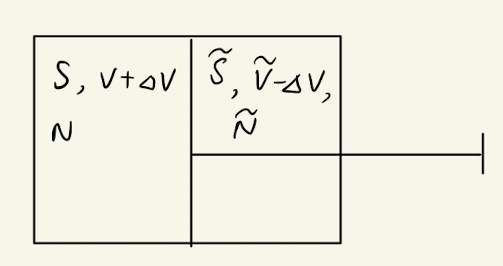
\includegraphics[width=0.8\textwidth]{images/0702-01.png}
	\caption{Composite system}
\end{figure}

Using the additivity postulate:
\begin{equation}
	\Delta U = U(S,V + \Delta V, N) + \tilde U (\tilde S, \tilde V - \Delta , \tilde N) -  (U(S,V,N)+U(\tilde S, \tilde V, \tilde N)) \geq 0
\end{equation}
The second term is the equilibrium energy, and it's minimised.

\textbf{Specialise to identical systems:}
\[ \tilde U = U \]
Then
\[ \Delta U = U(S,V+\Delta V, N )v+ U(S,V-\Delta V,N)-2U(S,V,N) \geq 0 \] 
For $ \Delta V  $ infinitesimal:
\[ \frac{\partial ^2 U}{\partial V^2} (\Delta V)^2 \] 
\[\implies \left( \frac{\partial ^2U}{\partial V^2} \right)_{S,N} \geq 0 \]
\[ dU = TdS -PdV +\mu dN\] 
\[ \frac{\partial U}{\partial V}_{S,V} = -P \] 
\[ \left( \frac{\partial ^2U}{\partial ^2} \right)_{S,N} = - \frac{1}{ \left ( \frac{\partial V}{\partial P} \right)_{S,V} } \] 
\[ = \frac{1}{V K_s} \geq 0 \] 
\begin{equation}
	K_s > 0
\end{equation}
where $ K_s $ is the isentropic compressibility. 

\subsection{Heat Transfer}
\[ \Delta U = U(S + \Delta S,V, N )v+ U(S - \Delta S,V,N)-2U(S,V,N) \geq 0 \] 
\[ \left (\frac{\partial ^2U}{\partial S^2} \right )_{V,N} \geq 0 \] 
\[ \left (\frac{\partial U}{\partial S} \right )_{V,N} = T \implies \] 
\[ \left (\frac{\partial ^2U}{\partial S^2} \right )_{V,N} = \left (\frac{\partial T}{\partial S} \right )_{V,N} = \left[ \left (\frac{\partial S}{\partial T} \right )_{V,N} \right]^{-1} ] \] 
\[ = \left[\frac{N}{T} \frac{T}{N}\left (\frac{\partial S}{\partial T} \right )_{V,N} \right ]^{-1} \geq 0\] 

\subsection{Volume Exchange for Helmholtz Free Energy}
\[ \Delta F = F(T,V+\Delta V, N) + F(T,V-\Delta V, N) -2F(T,V,N) \geq 0 \] 
\[ \left (\frac{\partial ^2F}{\partial V^2} \right )_{T,N} \geq 0  \] 
\[ \implies \left (\frac{\partial F}{\partial V} \right )_{T,N} = -P \] 
\[ \left (\frac{\partial ^2F}{\partial V^2} \right )_{T,N} = \left (\frac{\partial P}{\partial V} \right )_{T,N} = \left[ v \frac{1}{-v} \left (\frac{\partial V}{\partial P} \right )_{T,N} \right]^{-1}  \] 
\[ \frac{1}{VK_T} \geq 0 \] 
\[ \implies K_T \geq 0 \] 

\subsection{Heat Exchange for Enthalpy}
\[ H(S+\Delta S, P,N) + H(S-\Delta S, P,N) - 2H(S,P,N) \geq 0 \] 
\[ \implies \left (\frac{\partial ^2H}{\partial S^2} \right )_{P,N} \geq 0 \] 
\[ \left (\frac{\partial H}{\partial S} \right )_{P,N} = T \] 
\[ \left (\frac{\partial ^2H}{\partial S^2} \right )_{P,N} = \left[ \left (\frac{\partial S}{\partial T} \right )_{P,N} \right]^{-1} \geq 0 \] 
\[ \implies C_p \geq 0 \] 
\begin{shaded*}
	The stability conditions that we have derived so far are only valid for \textbf{extensive} variables!
\end{shaded*}
\subsection{What about intensive variables?}
We use TD relations.
\[ \left (\frac{\partial F}{\partial T} \right )_{V,N} = -S, \quad \left (\frac{\partial ^2F}{\partial T^2} \right )_{V,N} = - \left (\frac{\partial S}{\partial T} \right ) = \frac{-1}{\left (\frac{\partial ^2U}{\partial S^2} \right )_{V,N}} < 0\]
\[ \left (\frac{\partial U}{\partial S} \right )_{V,N} = T, \quad \left (\frac{\partial ^2U}{\partial S^2} \right )_{V,N} \] 
so
\begin{equation}
	\left (\frac{\partial ^2F}{\partial T^2} \right )_{V,N} < 0
\end{equation}

\subsection{Van der Waal's gas}
Ideal gas: \[ F = - Nk_bT\left[ ln (\frac{V}{N}) + \frac{3}{2}ln(k_BT) +X \right]  \] 
\textbf{Free, non-interacting particles} \\
Include interactions "treated crudely": \\

\begin{figure}[h]
	\centering
	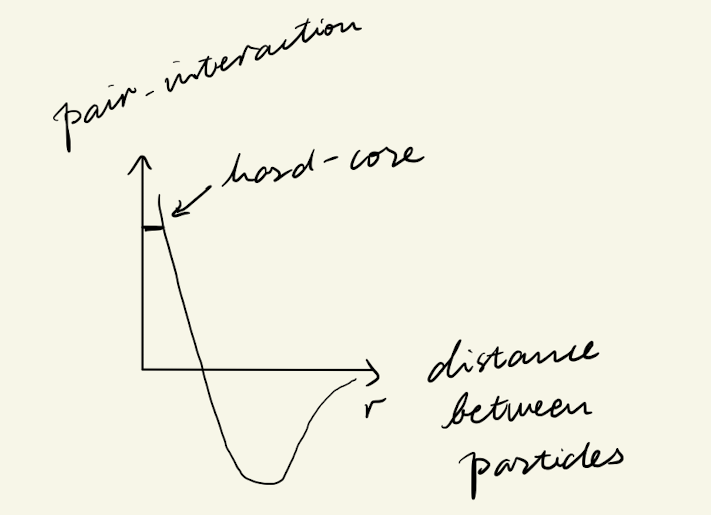
\includegraphics[width=0.8\textwidth]{images/0702-02.png}
	\caption{Van der Waal interaction model.}
	\label{fig:VDW}
\end{figure}
The interaction has two main effects:
\begin{enumerate}
	\item Energy is lowered by the mean interaction energy $ \propto \frac{N}{V}$ per particle.
	\item The hard-core potential restricts the volume to $ V \to V-Nb $ 
\end{enumerate}
\[ F_{VDW} = - Nk_BT \left[ ln(\frac{V-Nb}{N}) + \frac{3}{2} ln(k_BT) + X \right]  - a \frac{N^2}{V}\] 
where $ a $ (measure of attraction) and $ b $ (hard-core) are constants.
This is an extensive system, meaning we could use the Euler's equation. \\
\textbf{Pressure:} 
\[ P = - \left (\frac{\partial F}{\partial V} \right )_{T,N} =  \frac{Nk_BT}{V-Nb} + a \frac{N^2}{V^2} \] 

\begin{figure}[h]
	\centering
	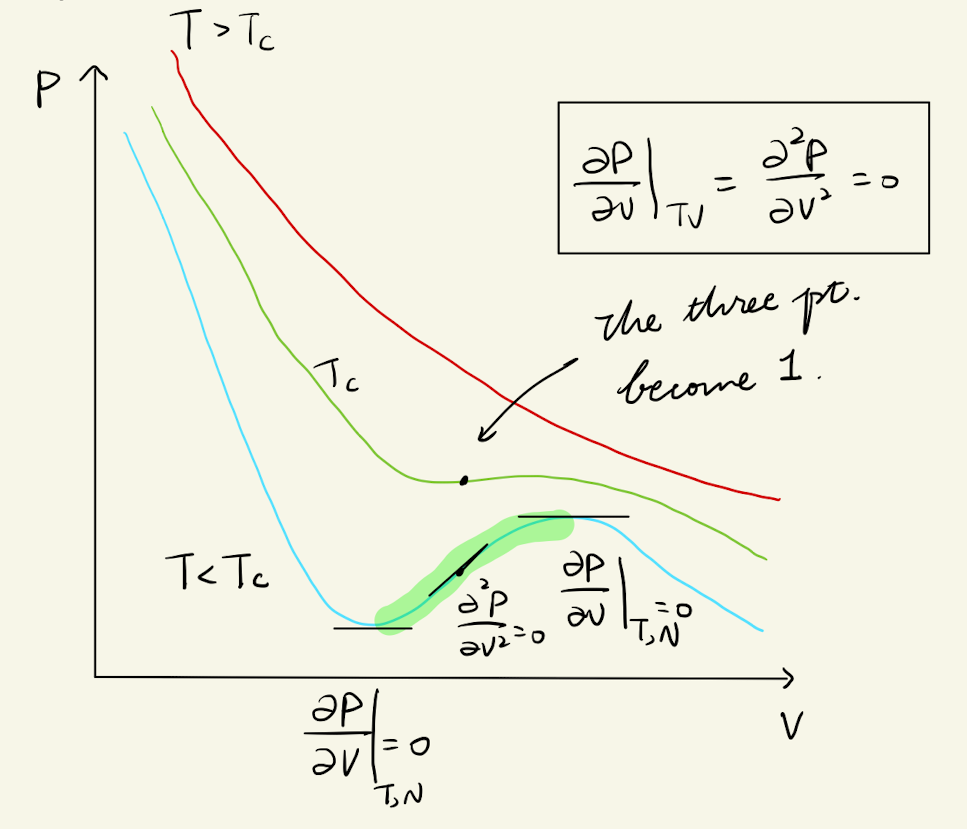
\includegraphics[width=0.8\textwidth]{images/0702-03.png}
	\caption{Pressure vs Volume diagram.}
	\label{fig:PvsV}
\end{figure}
\textbf{Stability:} 
\[ \left (\frac{\partial ^2F}{\partial V^2} \right )_{T,N} \geq \] 
\[ \left (\frac{\partial F}{\partial V} \right )_{T,N} = -P \] 
\[ \left (\frac{\partial ^2F}{\partial V^2} \right )_{T,N} = - \left (\frac{\partial P}{\partial V} \right )_T,N) > 0 \] 
\[ \implies  \left (\frac{\partial P}{\partial V} \right )_{T,N} < 0\] 
The highlighted part is unstable since $ \left (\frac{\partial P}{\partial V} \right )_{T,N} \geq 0 $.  \\

Want to calculate the critical temperature $ T_c $:

\[ \left (\frac{\partial P}{\partial V} \right )_{T,N} = 0 = \left (\frac{\partial ^2P}{\partial V^2} \right )_{T,N} = 0 \] 
\[ \frac{\partial P}{\partial V} = \frac{-Nk_BT}{(V_Nb)^2} + 2a \frac{N^2}{V^3} = 0\] 
\[ \implies Nk_BTV^3 = 2aN^2 (V-Nb)^2 \] 
\[  (\frac{\partial ^2P}{\partial V^2}   = \frac{2Nk_BT}{(V-Nb)^3} - 6a \frac{N^2}{V^{4}} = 0\] 
\[ \implies 2Nk_BTV^4 = 6aN^2(V-Nb)^3 \] 
Combine:
\[ 2V = 3(V-Nb) \] 
\begin{shaded*}
	\[ \implies V_c = 3Nb \] 
and
\[ k_BT_c = \frac{2aN^2(3Nb-Nb)^2}{N(3Nb)^3} =  \frac{8}{27}\frac{a}{b}\] 
\[ P_c = \frac{N_kBT}{V_c-Nb} - a \frac{N^2}{V_c^2} = \frac{1}{27}\frac{a}{b^2} \] 
\[ \frac{P_cV_c}{Nk_BT_c} = \frac{3}{8} \] Ideal gas: 1
\end{shaded*}
\end{document}

